\begin{figure}
\centering
\begin{subfigure}[b]{.49\textwidth}
    \centering
    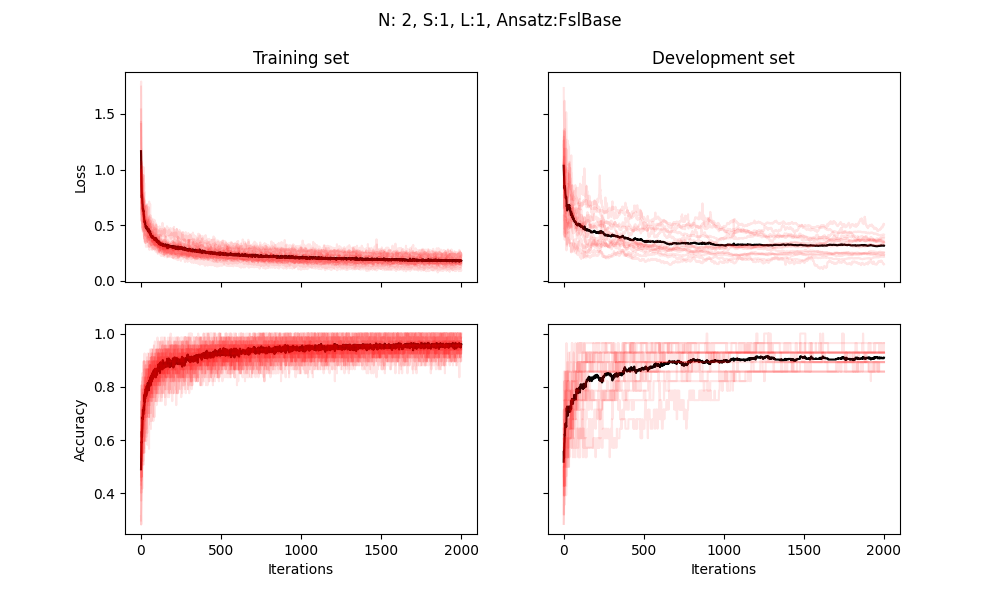
\includegraphics[width=\textwidth]{figures/single_model/FslBase/Epochs_2000--A_0.05--N_2--S_1--L_1--Ansatz_FslBase.png}
\end{subfigure}
\begin{subfigure}[b]{.49\textwidth}
    \centering
    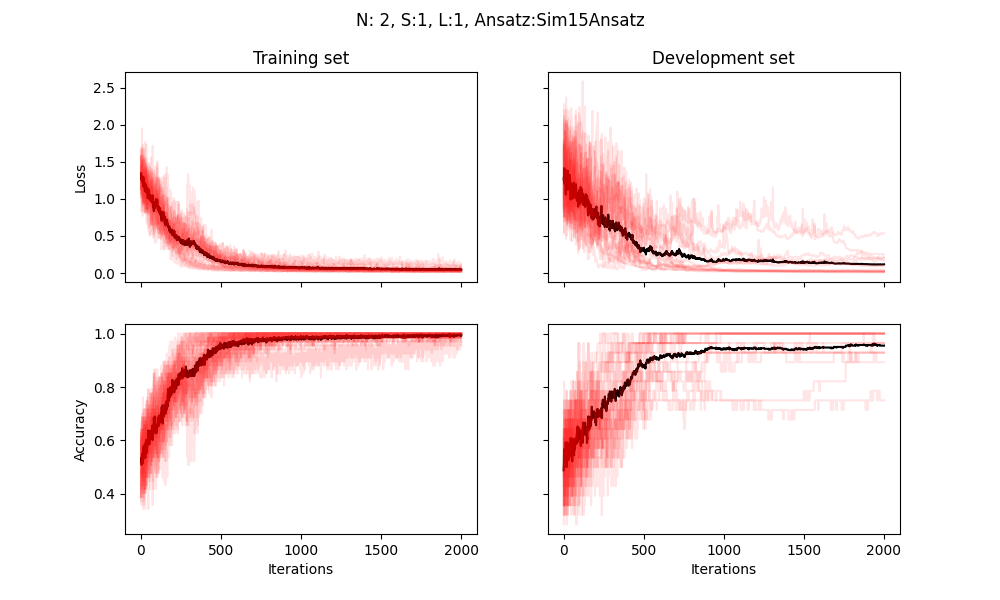
\includegraphics[width=\textwidth]{figures/single_model/Sim15Ansatz/Epochs_2000--A_0.05--N_2--S_1--L_1.png}
\end{subfigure}
\begin{subfigure}[b]{.49\textwidth}
    \centering
    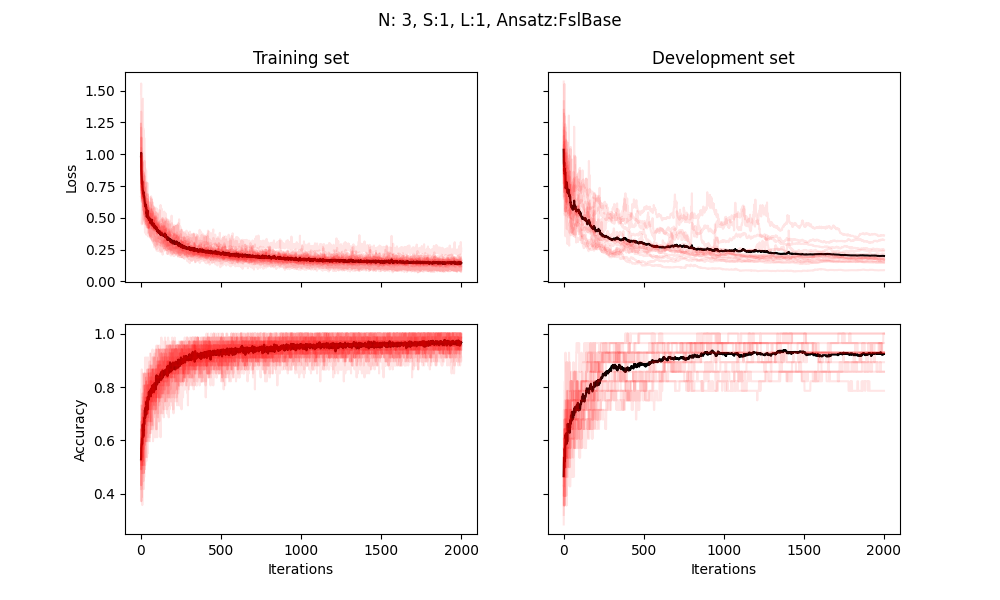
\includegraphics[width=\textwidth]{figures/single_model/FslBase/Epochs_2000--A_0.05--N_3--S_1--L_1--Ansatz_FslBase.png}
\end{subfigure}
\begin{subfigure}[b]{.49\textwidth}
    \centering
    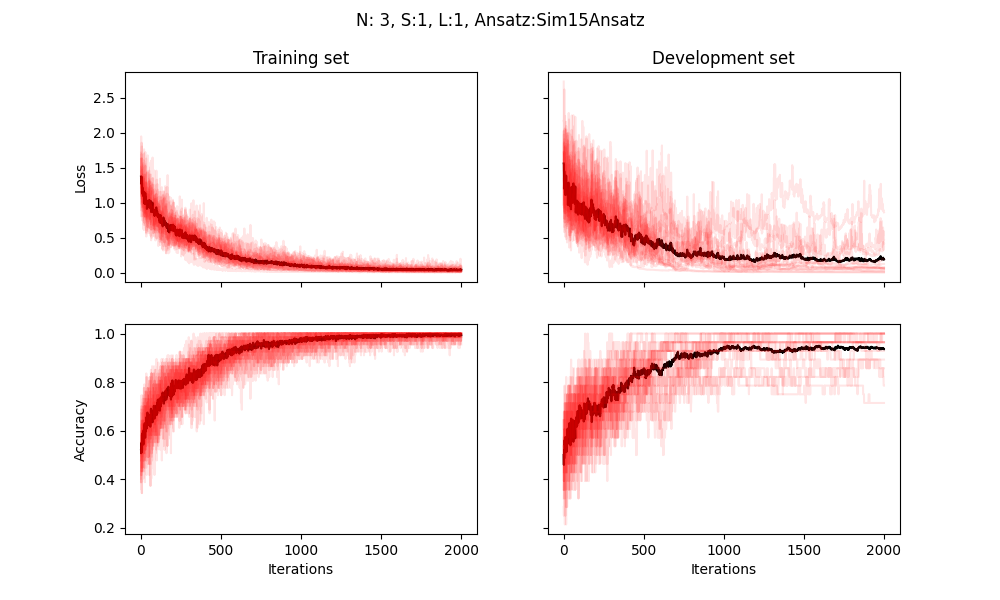
\includegraphics[width=\textwidth]{figures/single_model/Sim15Ansatz/Epochs_2000--A_0.05--N_3--S_1--L_1.png}
\end{subfigure}
\begin{subfigure}[b]{.49\textwidth}
    \centering
    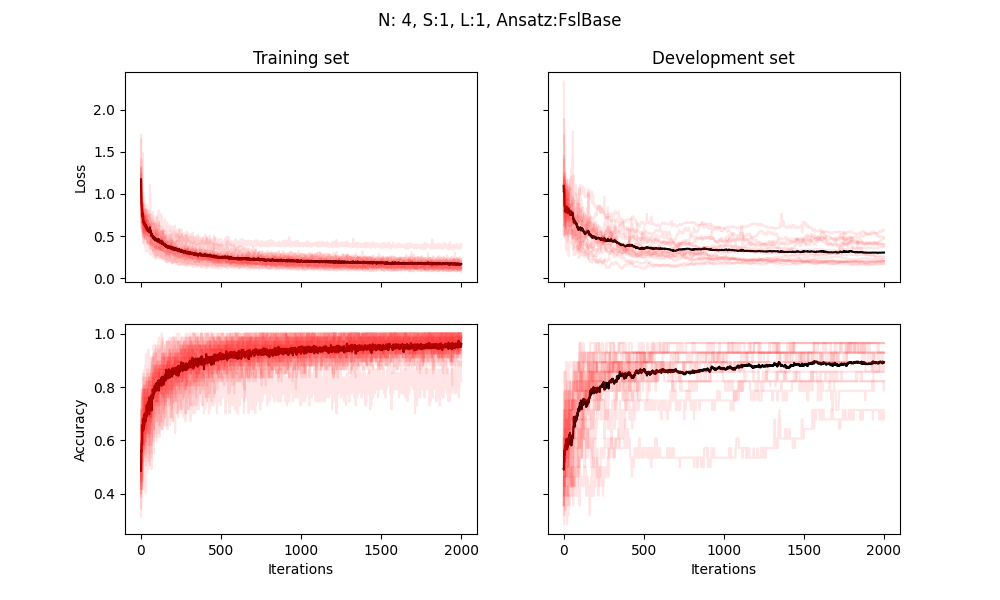
\includegraphics[width=\textwidth]{figures/single_model/FslBase/Epochs_2000--A_0.05--N_4--S_1--L_1--Ansatz_FslBase.png}
\end{subfigure}
\begin{subfigure}[b]{.49\textwidth}
    \centering
    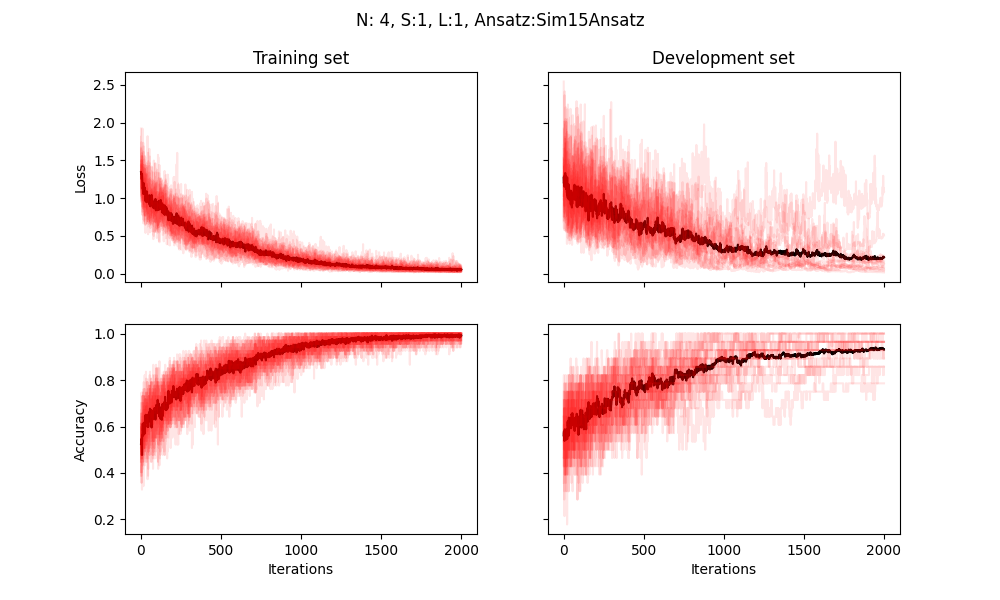
\includegraphics[width=\textwidth]{figures/single_model/Sim15Ansatz/Epochs_2000--A_0.05--N_4--S_1--L_1.png}
\end{subfigure}\\
\begin{subfigure}[b]{\textwidth}
    \centering
    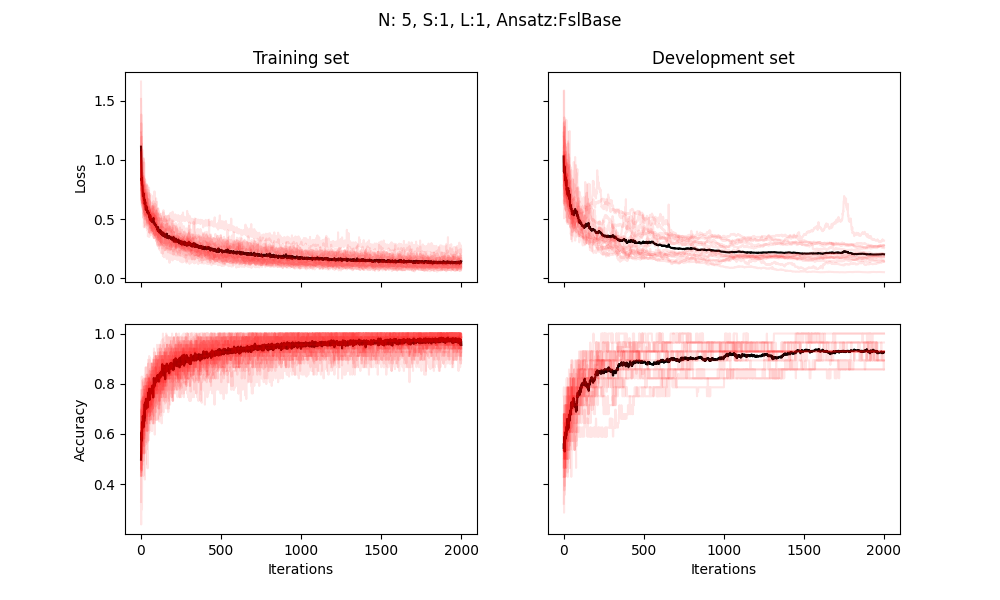
\includegraphics[width=0.5\textwidth]{figures/single_model/FslBase/Epochs_2000--A_0.05--N_5--S_1--L_1--Ansatz_FslBase.png}
\begin{subfigure}[b]{.49\textwidth}
    \centering
    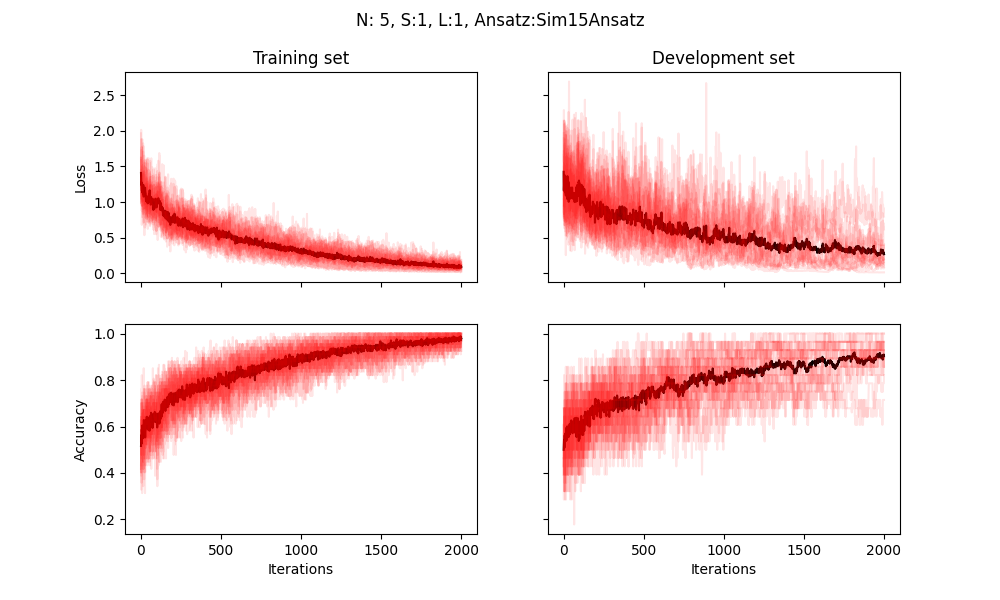
\includegraphics[width=\textwidth]{figures/single_model/Sim15Ansatz/Epochs_2000--A_0.05--N_5--S_1--L_1.png}
\end{subfigure}
\end{subfigure}
\caption[Spread of \mya for small datasets]{\label{fig:testspread} Training spread for two types of \mya on the MC task after, average in black and each run in red. On the left, FSL base and on the right Sim15.}
\end{figure}